\documentclass[12pt]{article}
\usepackage[margin=1in]{geometry}
\usepackage{amsmath}
\usepackage{amssymb}
\usepackage{graphicx}
\usepackage{parskip}

\title{\textbf{The Conjugate Gradient Method}}
\author{}
\date{}

\begin{document}

\maketitle

For applied scientific solving of linear systems, many accredit efficiency and speed to the
Conjugate Gradient Method of numerical analysis. Due to this fact, the Conjugate Gradient (CG)
Method is one of the most prominent iterative methods for solving sparse systems of linear
equations. In practice, the conjugate gradient method is an iterative algorithm that solves a
symmetric positive definite linear system $A\vec{x} = \vec{b}$ by minimizing the quadratic form
$\varphi(\vec{x}) = \tfrac{1}{2}\vec{x}^{\top} A \vec{x} - \vec{b}^{\top} \vec{x}$ along a sequence
of mutually $A$-conjugate search directions, converging in at most $n$ steps in exact arithmetic.

Analyzing the results produced from timing, one slope that speaks the loudest is the factoring and
solving of the SPD tridiagonal Poisson matrix for the CG method. For an average runtime of the
CG-Method, analysts broke it down to the big-oh of $\mathcal{O}(\sqrt{\kappa})$, where $\kappa$ is
the condition number of the given matrix $A$. In the worst case, a dense matrix akin to the SPD
tridiagonal Poisson represents $\kappa(A) = \mathcal{O}(N^{2})$, where CG needs
$\mathcal{O}(\sqrt{\kappa}) \approx \mathcal{O}(N)$, and sparse matrix-vector multiply occurs
iteratively for $\mathcal{O}(N)$ time, so $\mathcal{O}(N \cdot N)$ results in our final analysis of
$\mathcal{O}(N^{2})$ for the CG-Method. However, this is a merciful time, as BLAS-2 is highly
optimized for operations at $N \leq 1000$, so realistically the theoretical time is
$\mathcal{O}(N \cdot N^{2}) = \mathcal{O}(N^{3})$ for $N \geq 1000$. In the curve, it accurately
depicts this time, as the red curve (Dense-CG) paces the black curve ($\mathcal{O}(N^{2})$). This
is a great example to use, because it highlights one of the biggest problems with solving dense
PDEs as well as CG's biggest strength, that being sparsity in relation to a matrix's condition
number.

\begin{figure}[h]
    \centering
    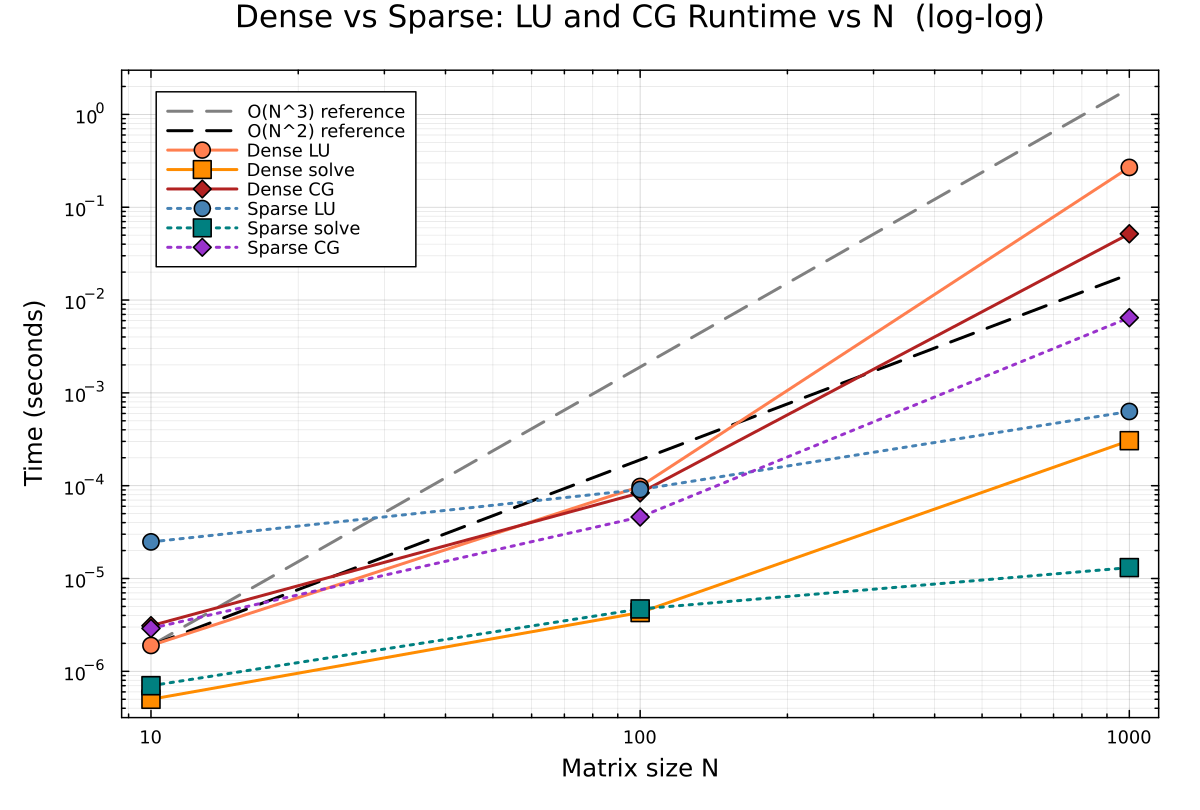
\includegraphics[width=0.85\textwidth]{dense_vs_sparse_timing.png}
    \caption{Runtime of the Conjugate Gradient method on the SPD tridiagonal Poisson matrix in
    both dense and sparse storage formats, plotted as a function of matrix size $N$ on a log-log
    scale. Reference lines for $\mathcal{O}(N^{2})$ (black, dashed) and $\mathcal{O}(N^{3})$
    (gray, dashed) are included for slope comparison, with sparse-format LU factorization and
    forward/back substitution timings shown alongside for context.}
    \label{fig:dense_vs_sparse_timing}
\end{figure}

\end{document}